% Template for PLoS
% Version 1.0 January 2009
%
% To compile to pdf, run:
% latex plos.template
% bibtex plos.template
% latex plos.template
% latex plos.template
% dvipdf plos.template

\documentclass[10pt]{article}

% amsmath package, useful for mathematical formulas
\usepackage{amsmath}
% amssymb package, useful for mathematical symbols
\usepackage{amssymb}

% graphicx package, useful for including eps and pdf graphics
% include graphics with the command \includegraphics
\usepackage{graphicx}

% cite package, to clean up citations in the main text. Do not remove.
%% \usepackage{cite}

\usepackage{color} 

% Use doublespacing - comment out for single spacing
\usepackage{setspace} 
%% \doublespacing

\usepackage[normalem]{ulem}

% Text layout
\topmargin 0.0cm
\oddsidemargin 0.5cm
\evensidemargin 0.5cm
\textwidth 16cm 
\textheight 21cm

% Bold the 'Figure #' in the caption and separate it with a period
% Captions will be left justified
\usepackage[labelfont=bf,labelsep=period,justification=raggedright]{caption}

% Use the PLoS provided bibtex style
%% \bibliographystyle{plos2009}
\usepackage[authoryear]{natbib}
\bibliographystyle{myunsrt}

% Remove brackets from numbering in List of References
\makeatletter
\renewcommand{\@biblabel}[1]{\quad#1.}
\makeatother


% Leave date blank
\date{}

\pagestyle{myheadings}
%% ** EDIT HERE **


%% ** EDIT HERE **
%% PLEASE INCLUDE ALL MACROS BELOW

%% END MACROS SECTION

\begin{document}

\begin{singlespace}
% Title must be 150 characters or less
\begin{flushleft}
{\Large 
\textbf{Assessment of Cancer Cell Line Representativeness using Microarrays for Merkel Cell Carcinoma}
}
% Insert Author names, affiliations and corresponding author email.
\\
Kenneth Daily$^{1}$,
Amy Coxon$^{1}$,
Jonathan S. Williams$^{1}$,
Chyi-Chia Richard Lee$^{2}$,
Daniel G. Coit$^{3}$,
Klaus J. Busam$^{4}$,
Isaac Brownell$^{1,5,\ast}$
\\

\bf{1} Dermatology Branch, National Cancer Institute, National Institutes of Health, Bethesda, MD, USA
\\
\bf{2} Laboratory of Pathology, National Cancer Institute, National Institutes of Health, Bethesda, MD, USA
\\
\bf{3} Department of Surgery, Memorial Sloan Kettering Cancer Center, New York, NY, USA
\\
\bf{4} Department of Pathology, Memorial Sloan Kettering Cancer Center, New York, NY, USA
\\
\bf{5} Dermatology Service, Department of Medicine, Memorial Sloan Kettering Cancer Center, New York, NY, USA
\\

$\ast$ E-mail: isaac.brownell@nih.gov

\end{flushleft}

\end{singlespace}

\section*{Abstract}
When using cell lines to study cancer, phenotypic similarity to the original tumor is paramount.
Yet, little has been done to characterize how closely Merkel cell carcinoma (MCC) cell lines model native tumors.
To determine their similarity to MCC tumor samples, we characterized MCC cell lines via gene expression microarrays.
Using whole transcriptome gene expression signatures and a computational bioinformatic approach, we identified significant differences between variant cell lines (UISO, MCC13, and MCC26) and fresh frozen MCC tumors.
Conversely, the classic WaGa and Mkl-1 cell lines more closely represented the global transcriptome of MCC tumors.
When compared to publicly available cancer lines, WaGa and Mkl-1 cells were similar to other neuroendocrine tumors, but the variant cell lines were not.
WaGa and Mkl-1 cells grown as xenografts in mice had histological and immunophenotypical features consistent with MCC, while UISO xenograft tumors were atypical for MCC.
Spectral karyotyping and short tandem repeat analysis of the UISO cells matched the original cell line's description, ruling out contamination.
Our results validate the use of transcriptome analysis to assess the cancer cell line representativeness and indicate that UISO, MCC13, and MCC26 cell lines are not representative of MCC tumors, whereas WaGa and Mkl-1 more closely model MCC.

\section*{Introduction}
Cancer cell lines are essential tools for modeling human malignancy.
However, many factors can alter the representativeness of a cultured cell line.
Some differences to the native tumor are expected with cells grown in culture due to the absence of vascular stroma and tumor architecture.
Additional discrepancies can arise due to the evolution of atypical subclones that possess \emph{in vitro} growth advantages, genomic instability associated with repeated passaging, alterations secondary to microbial infections in culture, and contamination from other cell lines \citep{Barallon2010Recommendation,CapesDavis2010Check}.
Phenotypic dissimilarity to the original tumor impacts the relevance of a cell line as an experimental model.
Thus, systematic comparison of cell lines to the cancers they are modeling is critical.

Microarray expression profiles have been used to compare cancer cell lines to native tumors for a number of cancer types \citep{Barretina2012Cancer,Carlson2007Quantitative,Wang2006Comparative,Gillet2011Redefining,Khan2001Classification,Li2008Genomic}.
In some cases, extensive transcriptomic differences were found between cell lines and primary tumors \citep{Li2008Genomic,Wang2006Comparative}.
These studies illustrate the utility of microarray expression profiling in characterizing cancer cell lines, however the implications of expression profile differences on the biological representativeness of cells lines were not assessed.

Merkel cell carcinoma (MCC) is an aggressive neuroendocrine skin cancer  \citep{Toker1972Trabecular,Maricich2009Merkel,Maricich2012Rodents}.
The risk of developing MCC is associated with ultraviolet light exposure, advanced age, and immunosuppression \citep{Hodgson2005Merkel,Becker2010Merkel}.
Approximately $80\%$ of MCC tumors have DNA of the Merkel cell polyomavirus (MCV) clonally integrated into their genome \citep{Feng2008Clonal}.
The MCV T antigen is thought to be important in MCC carcinogenesis \citep{Houben2010Merkel}, however, it is unclear if the presence or absence of integrated MCV alters the outcome or course of MCC.

Like most solid malignancies, diagnosis of MCC relies on histopathological examination of tumor tissue.
MCC shares a number of histopathological characteristics with other tumors of neuroendocrine origin.
For example, both MCC and small cell lung cancer (SCLC) are frequently composed of morphologically similar, small, round cells that frequently express chromogranin (CHGA), synaptophysin (SYP), and neuron-specific enolase (ENO2).
In contrast, immunostaining for cytokeratin 20 (KRT20) is more specific for MCC, whereas thyroid transcription factor 1 (TTF1) is a marker of SCLC \citep{Leech2001Merkel,Pulitzer2009Merkel}.

A growing number of MCC tumor cell lines are available \citep{Krasagakis2001Growth,Leonard1993Characterization,Rosen1987Establishment,Leonard1995Characterisation,Moll1994Establishment,Ronan1993Merkel}.
Most MCC cell lines grow in suspension, express MCC immunomarkers, and demonstrate dense core granules on ultrastructural analysis.
MCC cell lines with these typical features, such as WaGa and Mkl-1, are termed ``classic'' \citep{Ronan1993Merkel,Leonard1993Characterization,VanGele2004Geneexpression}.
In contrast, "variant" MCC cell lines like UISO-MCC-1 (henceforth referred to as UISO) \citep{Ronan1993Merkel}, \uline{MCC13, and MCC26} \citep{Leonard1995Characterisation} grow adherently in culture, lack typical markers on immunostaining, and have reduced numbers of neurosecretory granules.
The majority of classic MCC cell lines test positive for MCV, whereas most variant cell lines are MCV negative. 
Little has been done to assess the representativness of \uline{either classic or variant MCC cell lines.}

Here we apply computational and experimental methods to compare MCC cell line transcriptomes to each other, to fresh tumor tissue, and to other cancer cells in order to examine their representativeness.
Using these approaches, we find that \uline{three variant cell lines are not characteristic of MCC} whereas three classic MCC cell lines more closely represent native MCC tumors. 
We validate the non-representative biology of UISO cells by demonstrating atypical \emph{in vivo} growth in a xenograft tumor model. 

\section*{Results}

\subsection*{Variant cell lines clusters distinctly from MCC tumors and classic MCC cell lines}
In order to test how well they modeled MCC, we analyzed global RNA expression in six MCC lines: \uline{the variant lines UISO, MCC13, and MCC26,} and the classic lines WaGa \citep{Houben2010Merkel}, Mkl-1 \citep{Rosen1987Establishment}, and a newly established MCC cell line SK-MC01 (hereafter MC01).
We also analyzed global RNA expression from 23 MCC and 9 SCLC fresh frozen tumor samples.

We performed hierarchical clustering to identify groups of samples with similar global gene expression profiles (Figure \ref{fig:clustering}A).
The \uline{variant cell line samples} formed a group divergent from the MCC tumors, SCLC tumors, and the classic WaGa, Mkl-1, and MC01 samples, indicating that these cell lines are distinct from both native tumors and the more typical MCC cells.
\uline{Furthermore, the UISO samples clustered separately from the other variant cell lines, MCC13 and MCC26.}
In contrast to the variant lines, WaGa, Mkl-1, and MC01 cells clustered with the MCC tumor samples.
These differences in gene expression can also be visualized in a principal components analysis (PCA) projection (Figure \ref{fig:clustering}B, Figure S1).
In the PCA, expected differences due to \emph{in vitro} growth appear to contribute to the separation between cultured cells and fresh frozen tumor samples along the second principal component.

\subsection*{Global gene expression differences between the MCC cell lines and tumor samples}
To identify RNA expression differences, we performed differential expression analysis between the MCC tumor samples and each group of cell lines: \uline{classic (WaGa, Mkl-1, and MC01), variant (MCC13 and MCC16), and} UISO.
Figure \ref{fig:venn} depicts a Venn diagram of the differentially expressed probe sets in the comparison of each group to the tumor samples.
In total, 1023 probe sets showed common differential expression between the tumor samples and all three groups.
In line with our prior results, many more probe sets were uniquely differentially expressed between the MCC tumor samples and UISO cells \uline{(4223) or the other variant lines (4103)} than between the MCC tumors and \uline{the classic cell lines (938)}.
To quantify the overall similarity of cell line expression profiles to MCC tumor samples, Spearman's rank correlation coefficients between individual expression profiles of MCC cell lines and tumor samples were computed (Figure S2).
\uline{The classic} samples were similar to tumor samples (median correlation $=0.83$).
UISO cells were less similar (median correlation $=0.66$), \uline{as were the other variant lines (median correlation $=0.68$).}

\subsection*{Virus status of MCC tumors does not influence gene expression comparisons}
Despite having varied clinical features, the MCC tumor samples analyzed in this study were remarkably homogeneous at the RNA expression level.
We observed no significantly differentially expressed probe sets when comparing samples based on clinically relevant phenotypes such as tumor site (primary skin vs. metastasis), if the patient ultimately had a recurrence, or tumor stage (stage 1-2 vs. Stage 3, coded as early vs. late; Table S1).
\uline{We found relatively few (214) significantly differentially expressed probe sets between MCV positive and negative tumors (Table S2), including previously described differences in TP53 and RB1 expression \cite{Waltari2011Association,Sihto2011Merkel,Bhatia2010Merkel}.
Consistent with this high degree of similarity, there was little difference in the correlation values for each cell line when compared independently to MCV positive or MCV negative tumors (Table S3).}
These observations suggest that clinical differences and MCV status are not driving the divergent expression profile observed in the MCV-negative \citep{Guastafierro2013Characterization} \uline{variant cell lines.}

\subsection*{Predicted functional differences between MCC cell lines and tumor samples}
Having identified significant differences between the variant MCC cell lines and the tumor samples at the single gene level, we sought to identify functional differences at the pathway level.
To identify pathways that are significantly differentially expressed between MCC cell lines and tumor samples, we applied Gene Set Enrichment Analysis (GSEA) \citep{Subramanian2005Gene} using the differential expression data and pathway gene sets taken from the Kyoto Encyclopedia of Genes and Genomes (KEGG) database \citep{Kanehisa2000KEGG}.
\uline{We assessed pathway enrichment in the differentially expressed genes comparing MCC tumors to UISO cells, variant cell lines, and classic cell lines (Table S4).}


Although enrichment of any given pathway requires experimental validation, GSEA analysis often accurately reveals biological schemes.
It is therefore noteworthy that the gene expression differences between UISO cells and MCC tumors show concordant changes in processes central to oncogenesis such as DNA replication and RNA processing (spliceosome).
Despite having a similarly large number of differentially expressed probe sets as UISO, \uline{the other variant cell lines had very few differentially expressed pathways, with only the proteasome pathway showing high enrichment.}
On the other hand, highly differentially expressed pathways between MCC tumors and the classic cell lines could be attributed to cultured cells lacking both stromal interactions (focal adhesion and ECM interactions) and an immune infiltrate (multiple autoimmune, inflammatory, and infectious pathways).
Taken together, the GSEA results further suggest that UISO cells are less appropriate to use as a model for MCC, \uline{but give little insight into the large differences between MCC tumors and the other variant cell lines.}

\subsection*{Classification of MCC cell lines using tumor samples}
Since our analyses suggested that variant cell lines were similarly distinct from both skin and lung neuroendocrine tumors, we sought to test if the variant lines would be classified as MCC or SCLC using a random forest machine learning classifier trained on expression signatures of the fresh frozen tumor samples (see Supplementary Methods).
This classifier was applied to the expression signatures of the MCC cell lines.
The trained model strongly classified all \uline{classic} cell lines as MCC (over 80\% probability, Table \ref{tab:classifier}). 
\uline{None of the variant cell lines were} strongly classified as MCC or SCLC, indicating they resemble SCLC as much as they resemble MCC.

\subsection*{Classification of MCC cell lines using the Cancer Cell Line Encyclopedia}
Since the gene expression of \uline{variant cell lines} did not resemble MCC tumors or more typical classic MCC cell lines, we assessed their distinctness using data from the Cancer Cell Line Encyclopedia (CCLE)\citep{Barretina2012Cancer} to compare MCC cell line expression data to a broad set of cancer cell lines.
We selected a set of eight cancer types from the CCLE that were common malignancies or shared some feature with MCC (from the skin, neuroendocrine, or neuroectodermal) to analyze with the MCC cell lines.


A random forest classifier was constructed using the selected CCLE lines and the Mkl-1 and WaGa cell lines (grouped as an MCC class) to classify the variant cell lines (see Supplementary Methods).
The resulting random forest did not classify the UISO samples as MCC (1\% probability).
They were classified with nearly equal probability for a number of tumor types, including melanoma, hepatocellular, breast, and lung carcinomas (Table S5).
The variant samples MCC13 and MCC26 were classified more strongly as MCC (up to 18\% probability), but were similarly classified to other cancer types as UISO.
Held out WaGa or Mkl-1 samples were strongly classified as MCC (70\% probability, Table S6).
Using PCA visualization, we observed that WaGa and Mkl-1 samples clustered near neuroendocrine (SCLC) and neuroectodermal (Ewing’s sarcoma) samples. 
As expected, UISO samples clustered away from the neuroendocrine tumors, while the MCC13 and MCC26 samples cluster in between the UISO and classic samples (Figure \ref{fig:pcaccle}).
These findings reinforce that UISO, MCC13, and MCC26 do not resemble typical MCC cell lines.

\subsection*{Immunohistochemical analysis of MCC xenograft tumors}
To confirm that the distinct expression profile observed in cultured UISO cells correlates with an atypical tumor phenotype \emph{in vivo}, we grew xenograft tumors with UISO, WaGa, and Mkl-1 cells in immunocompromised mice.
Histologically, WaGa tumors showed features consistent with MCC: sheets of tumor cells with scant cytoplasm, rounded nuclei, inconspicuous nucleoli, stippled chromatin patterning, and a brisk mitotic rate (Figure \ref{fig:ihc}).
WaGa xenograft tissue also resembled the immunophenotype of typical MCC tumors with positive immunostainng for the neuroendocrine markers chromogranin, NCAM1 (CD56), and ENO2.
The MCC marker KRT20 and pan-cytokeratin (AE1/AE3) both stained with a characteristic paranuclear dot pattern in WaGa tumors, and the SCLC marker TTF1 was negative.
As a MCV positive cell line \citep{Houben2010Merkel}, WaGa xenografts stained with CM2B4, an anti-MCV T antigen antibody.
Mkl-1 tumors showed immunohistochemical features similar to WaGa tumors, consistent with typical MCC tumors (data not shown).

In contrast, UISO xenografts did not resemble typical MCC tumors.
The UISO tumors had abundant fibrovascular stroma separating islands of tumor cells with large, irregular, hyperchromatic nuclei, irregular dendritic processes, and perinuclear clearing.
UISO tumors lacked staining for MCC markers such as chromogranin, KRT20, and pan-cytokeratin.
However, there was focal staining for NCAM1 and ENO2.
Staining for TTF1 and CM2B4 were negative, as expected.
Staining was also negative for S100, CD34, and KRT7 (data not shown).
Overall, UISO xenograft tumors were not diagnostic for MCC and were most consistent with a poorly-differentiated neuroendocrine tumor possessing sarcomatoid features.

\subsection*{The UISO cell line is not contaminated}
Cross contamination with another cancer cell line could explain why UISO cells are not representative of MCC.
Fortunately, early cytogenetic characterizations of UISO cells and the availability of low-passage cells allowed us to confirm the provenance of the contemporary cell line.
We performed spectral karyotyping (SKY) on UISO cells to compare with previously reported cytogenetic changes \citep{VanGele2002Combined,VanGele1998Characteristic}.
On metaphase spreads, several recurrent chromosomal changes were identified consistent with prior studies, including a small insertion at 1p36.2, a cryptic insertion or duplication on 6q, a dicentric chromosome 8, and a small heterogeneous ring chromosome (Figure \ref{fig:sky}).
A new t(10;19) translocation was also observed.
Conservation of these features strongly supports the present day cell line being of the same origin as the UISO cells used in earlier publications.

To confirm this, we obtained archived early passage cells directly from the laboratory that established the UISO cell line \citep{Ronan1993Merkel}.
Short tandem repeat (STR) profiling \citep{Masters2001Short} was performed using 16 markers (see Supplementary Methods) on all of the MCC cell lines used here.
The STR fingerprint of the UISO cell line was identical to the early passage UISO cells (Table S7).
Moreover,  none of the cell lines were similar to any cell line available in the major cell line databases (ATCC, DSMZ, JCRB), indicating no cross contamination with an STR characterized cell line occurred.

\section*{Discussion}

Characterization of tumor cell lines is important in developing appropriate and representative \emph{in vitro} models for the study of cancer.
Here we found that \uline{three variant MCC cell lines} were not representative of MCC tumors based on multiple comparative analyses of global gene expression and predicted gene set function.
Furthermore, machine learning approaches failed to classify UISO cells as MCC, whereas other variant cell lines were more similar to classic lines, but were not strongly classified as MCC.
UISO also had an atypical histopathologic phenotype when grown as xenograft tumors in mice.
At the same time, we found that the WaGa and Mkl-1 cell lines more closely resembled MCC tumors in gene expression and \emph{in vivo} growth.


In light of these findings, we speculate that an atypical MCC tumor gave rise to the UISO cell line.
UISO cells were derived from a tumor arising on the thigh of a patient much younger than the mean age for MCC presentation (46 versus 72 years) \citep{Ronan1993Merkel}.
The primary tumor uncharacteristically failed to show chromogranin and MAK-6 pan-cytokeratin staining, but did have ENO2 and focal CAM5.2 staining.
KRT20 staining was not assessed, as the antibody was not in widespread use at the time.
This immunophenotype in a skin tumor is consistent with MCC, but would not be considered diagnostic by today's standards.
We found UISO xenografts to be chromogranin negative, cytokeratin negative by AE1/AE3 staining, negative for KRT20 staining, and possessing sarcomatoid histologic features.
The focal NCAM1 and ENO2 staining in UISO xenografts were consistent with a neuroendocrine tumor, possibly a poorly differentiated MCC.
UISO xenograft tumors did express CD99 (data not shown), which is seen in peripheral primitive neuroectodermal tumors.
However, UISO cells did not have the canonical t(11;22)(q24;q12) translocation associated with primitive neuroectodermal tumors (Figure \ref{fig:sky} and data not shown)\citep{TurcCarel1988Chromosomes}.
Given the atypical nature of UISO’s tumor of origin, it is not surprising that the cell line is atypical and possesses a transcriptome and \emph{in vivo} biology that is non-representative of MCC tumors in general.

An atypical tumor of origin may not account for all the uncharacteristic features of UISO \uline{or other variant MCC cell lines.}
Even in typical MCC tumors, a minority sub-population of aberrant cells could exhibit a selective growth advantage in culture.
A cell line derived from such cells would not reflect the average gene expression or biology of MCC tumors.
In such a scenario, the sub-population cells could still be biologically important to tumor behavior, and having a cell culture model of the atypical cells could potentially be instructive.
Therefore, the UISO cell line and other non-representative cell lines may still prove useful in the study of cancer biology.

In contrast to \uline{the variant lines,} WaGa and Mkl-1 cells were more representative of MCC tumors.
Expression differences relative to tumor tissue did exist with WaGa and Mkl-1 cells, which are expected due to the lack of stroma, vasculature, and hematopoietic cells in cultured cancer cells.
As a model system to study the biology of MCC and predict the behavior of native tumors, it appears that WaGa and Mkl-1 are preferable to UISO \uline{or other variant lines.}

A previous study comparing MCC cell lines using expression microarrays with only 1083 genes found that UISO cells clustered with classic MCC lines, such as Mkl-1 \citep{VanGele2004Geneexpression}.
The limited scope of the genes analyzed and the lack of MCC tumor samples likely contributed to \uline{this finding that conflicts with our results.}
In contrast, using a comprehensive set of more than 40,000 human transcripts, we have demonstrated through multiple analyses that UISO samples cluster separately from both classic cell lines as well as MCC tumor samples.

It is interesting to note that on a transcriptome level, the set of MCC tumor samples analyzed in this study are quite homogeneous.
Clustering of the expression data failed to identify subclasses of MCC with strongly distinct gene expression signatures.
\uline{We identified few differences in gene expression between MCV positive and negative tumor samples.}
This contrasts with a recent publication comparing virus-positive and virus-negative MCC tumors in which many more significant differences were found \citep{Harms2013Distinct}.
The reason for these differing results is unknown.
However, in their study, only 46\% of the tumors analyzed were found to be virus positive, whereas most reports indicate 70-80\% of MCC tumors are virus positive \citep{Pulitzer2009Merkel,Feng2008Clonal}.
This is more consistent with the 87\% virus positive tumors we observed here.
It is not clear if this reflects a difference in virus detection methods, or a true difference in the patient populations.
Regardless, there was no concordance between the virus status of the tumors and their dissimilarity to the variant cell lines or their similarity to WaGa and Mkl-1, indicating that the differences observed \uline{in the variant cell lines} are not driven by viral status.

The independence of tumor viral status on cell line similarity is an important observation, as variant MCC cell lines are predominantly MCV-negative, and classic lines tend to be MCV-positive. 
All three variant cell lines used in this study are MCV-negative, whereas the classic lines are MCV-positive.
By definition, variant lines lack expression of certain differentiation markers, and our data suggest that variant cell lines may be divergent from MCC tumors on a more general level. 
However, the fact that MCV-negative native tumors are not similarly distinct from MCV-positive tumors and classic MCC cell lines suggests that MCV status alone is not the driver of atypical gene expression in the variant cell lines.

We have demonstrated that the question of cell line representativeness can be answered (in part) by the use of gene expression microarray data.
Straightforward computational methods and publicly available data can be applied to compare cell lines with native tumor tissue and other cell lines to assess cancer type concordance.
These types of techniques can, and should, be applied when using existing lines or developing a new one.
With respect to MCC, our analysis suggests that representative cell lines such as WaGa or Mkl-1 should be favored over UISO\uline{, MCC13, or MCC16} as an \emph{in vitro} experimental model.

\section*{Materials and Methods}

\subsection*{MCV detection by real time quantitative PCR}

Primers were designed to amplify a region of the MCV T antigen (coordinates 444-579 in the ``MCV350'' sequence GenBank Accession EU375803) to detect MCV DNA in MCC tumor samples by qPCR.
\uline{Primers for $\beta$-actin (\emph{ACTB}), a gene on chromosome 17,} were used as a reference on all MCC tumor samples.

\subsection*{Cell lines}
The MCC cell lines Mkl-1 \citep{Rosen1987Establishment}, WaGa \citep{Houben2010Merkel}, and UISO \citep{Ronan1993Merkel}, and MCC13 and MCC26 \citep{Leonard1995Characterisation} have been described previously.
SK-MC01 cells were generated at the Memorial Sloan Kettering Cancer Center (MSKCC).

\subsection*{cDNA array hybridization of tumor samples and cell lines}
Fresh frozen tumor specimens were supplied by the MSKCC tumor bank.
Total RNA was extracted from tumor specimens and hybridized to Human Genome U133A 2.0 Array (Affymetrix) GeneChips.

Total RNA was extracted from three to six replicates of each cell line (single replicate of MC01) and hybridized to the Human Genome U133A 2.0 Array (Affymetrix).
Three replicates of all cell lines (excluding MC01) were also hybridized to the GeneChip Human Genome U133 Plus 2.0 Array (Affymetrix).

\subsection*{Microarray analysis}
For MCC tumors, SCLC tumors, and MCC cell lines on the Affymetrix U133A 2.0 platform, normalization, filtering, and analysis of microarray expression data were performed using R (details in Supplemental Methods).
Raw CEL files for CCLE data were downloaded directly from GEO (accession GSE36133) and were normalized as above with MCC cell line Affymetrix U133 Plus 2.0 array data.
We call probe sets to be differentially expressed at a fold change $>= 2$ and $q <= 0.05$.

\subsection*{Classification of MCC cell lines with MCC and SCLC tumors}
A random forest classifier was trained using the microarray expression data for the 23 MCC and 9 SCLC tumor samples.
The classifier was then applied to the MCC cell lines, and the average class prediction was determined for each of the MCC cell lines across sample replicates.

\subsection*{Classification of MCC cell lines with CCLE cell lines}
A random forest classifier was trained using the microarray expression data for MCC cell lines (except for UISO) along with samples from the CCLE dataset.
The classifier was then applied to the variant (UISO, MCC13, and MCC26) samples.

\subsection*{STR Profiling}
Genomic DNA was isolated from all cell lines and sent to the Johns Hopkins Fragment Analysis Facility for STR profiling on all cell lines except MCC13 and MCC26 using the AmpF$\ell$STR Identifiler PCR Amplification Kit (Applied Biosystems), which profiles 16 STR markers (Table S7). MCC13 and MCC26 were profiled using the Promega PowerPlex 18D Kit, which profiles the same 16 markers plus two others.

\subsection*{Mouse xenografts}
Five to eight-week-old female NOD/scid mice were obtained from the NCI Animal Production Program and housed under specific pathogen-free conditions.
Tumors were induced by subcutaneous injection of $10^7$ WaGa cells, $2\mathrm{x}10^7$ Mkl-1 cells, or $10^6$ UISO cells in $200\mu\mathrm{L}$ sterile saline into the posterior lateral flank of the mice.
Tumor tissue was collected and fixed in neutral buffered formalin after tumors were clinically detectable.

\subsection*{Immunohistochemistry of mouse xenograft tumors}
Paraffin-embedded tissue sections (5 $\mu\mathrm{m}$) of fixed xenograft tumors on glass slides were stained on an automated immunostainer (Ventana Medical System), according to the manufacturer's instructions.
The primary antibodies and antigen retrieval methods used are indicated in Table S8.

\subsection*{Spectral karyotyping of the UISO cell line}
UISO cells were harvested after Colcemid (Life Technologies) treatment ($0.025 \mu\textrm{g/mL}$: 1–2 hours) and processed by standard cytogenetic methods.
Breakpoints on the SKY-painted chromosomes were determined by comparison with corresponding inverted DAPI banding.
We report SKY results by using the International System for Human Cytogenetic Nomenclature (ISCN, 2013).

\subsection*{Data access}
All tumor sample and cell line microarray data have been deposited in NCBI's Gene Expression Omnibus \citep{Edgar2002Gene} and is accessible through GEO Series accession number GSE50451.
All analysis code, including generation of all figures, tables, and supplementary tables and figures, are available in reference \cite{DailyUISOReproducible2014} (DOI 10.6084/m9.figshare.1030618).
See the Supplementary Methods for details.

\section*{Conflicts of Interest}
The authors state no conflict of interest.

\section*{Acknowledgments}
This research was supported by the NIH Intramural Research Program, Center of Cancer Research, National Cancer Institute.
Its contents are solely the responsibility of the authors and do not necessarily represent the official views of the NIH.
We thank the NCI CCR Informatics Core for assistance.
We thank Dr. Tapas K. Das Gupta for providing early passage UISO cells.
We thank Dr. Patrick Moore and Dr. J\"{u}rgen Becker for providing WaGa, Mkl-1, and late-passage UISO cells.
We thank Dr. Patrick Moore for providing MCC13 and MCC26 cells.
We thank Dr. Jedd Wolchock for assistance in generating SK-MC01 cells.
We thank Dr. Mark Raffeld and Cindy Harris for immunohistochemical assays.
We thank Dr. Anna Roschke and Kenneth Nakahara for the SKY analysis.
We thank Dr. Sean Davis for critical reading of the manuscript and methodological insights.

This study utilized the high-performance computational capabilities of the Biowulf Linux cluster at the NIH (http://biowulf.nih.gov).

\section*{References}
\begin{singlespace}
\bibliography{uisopub,extra}
\end{singlespace}

\newpage

\section*{Figure Legends}

\begin{figure}[!ht]
  \begin{center}
    %% 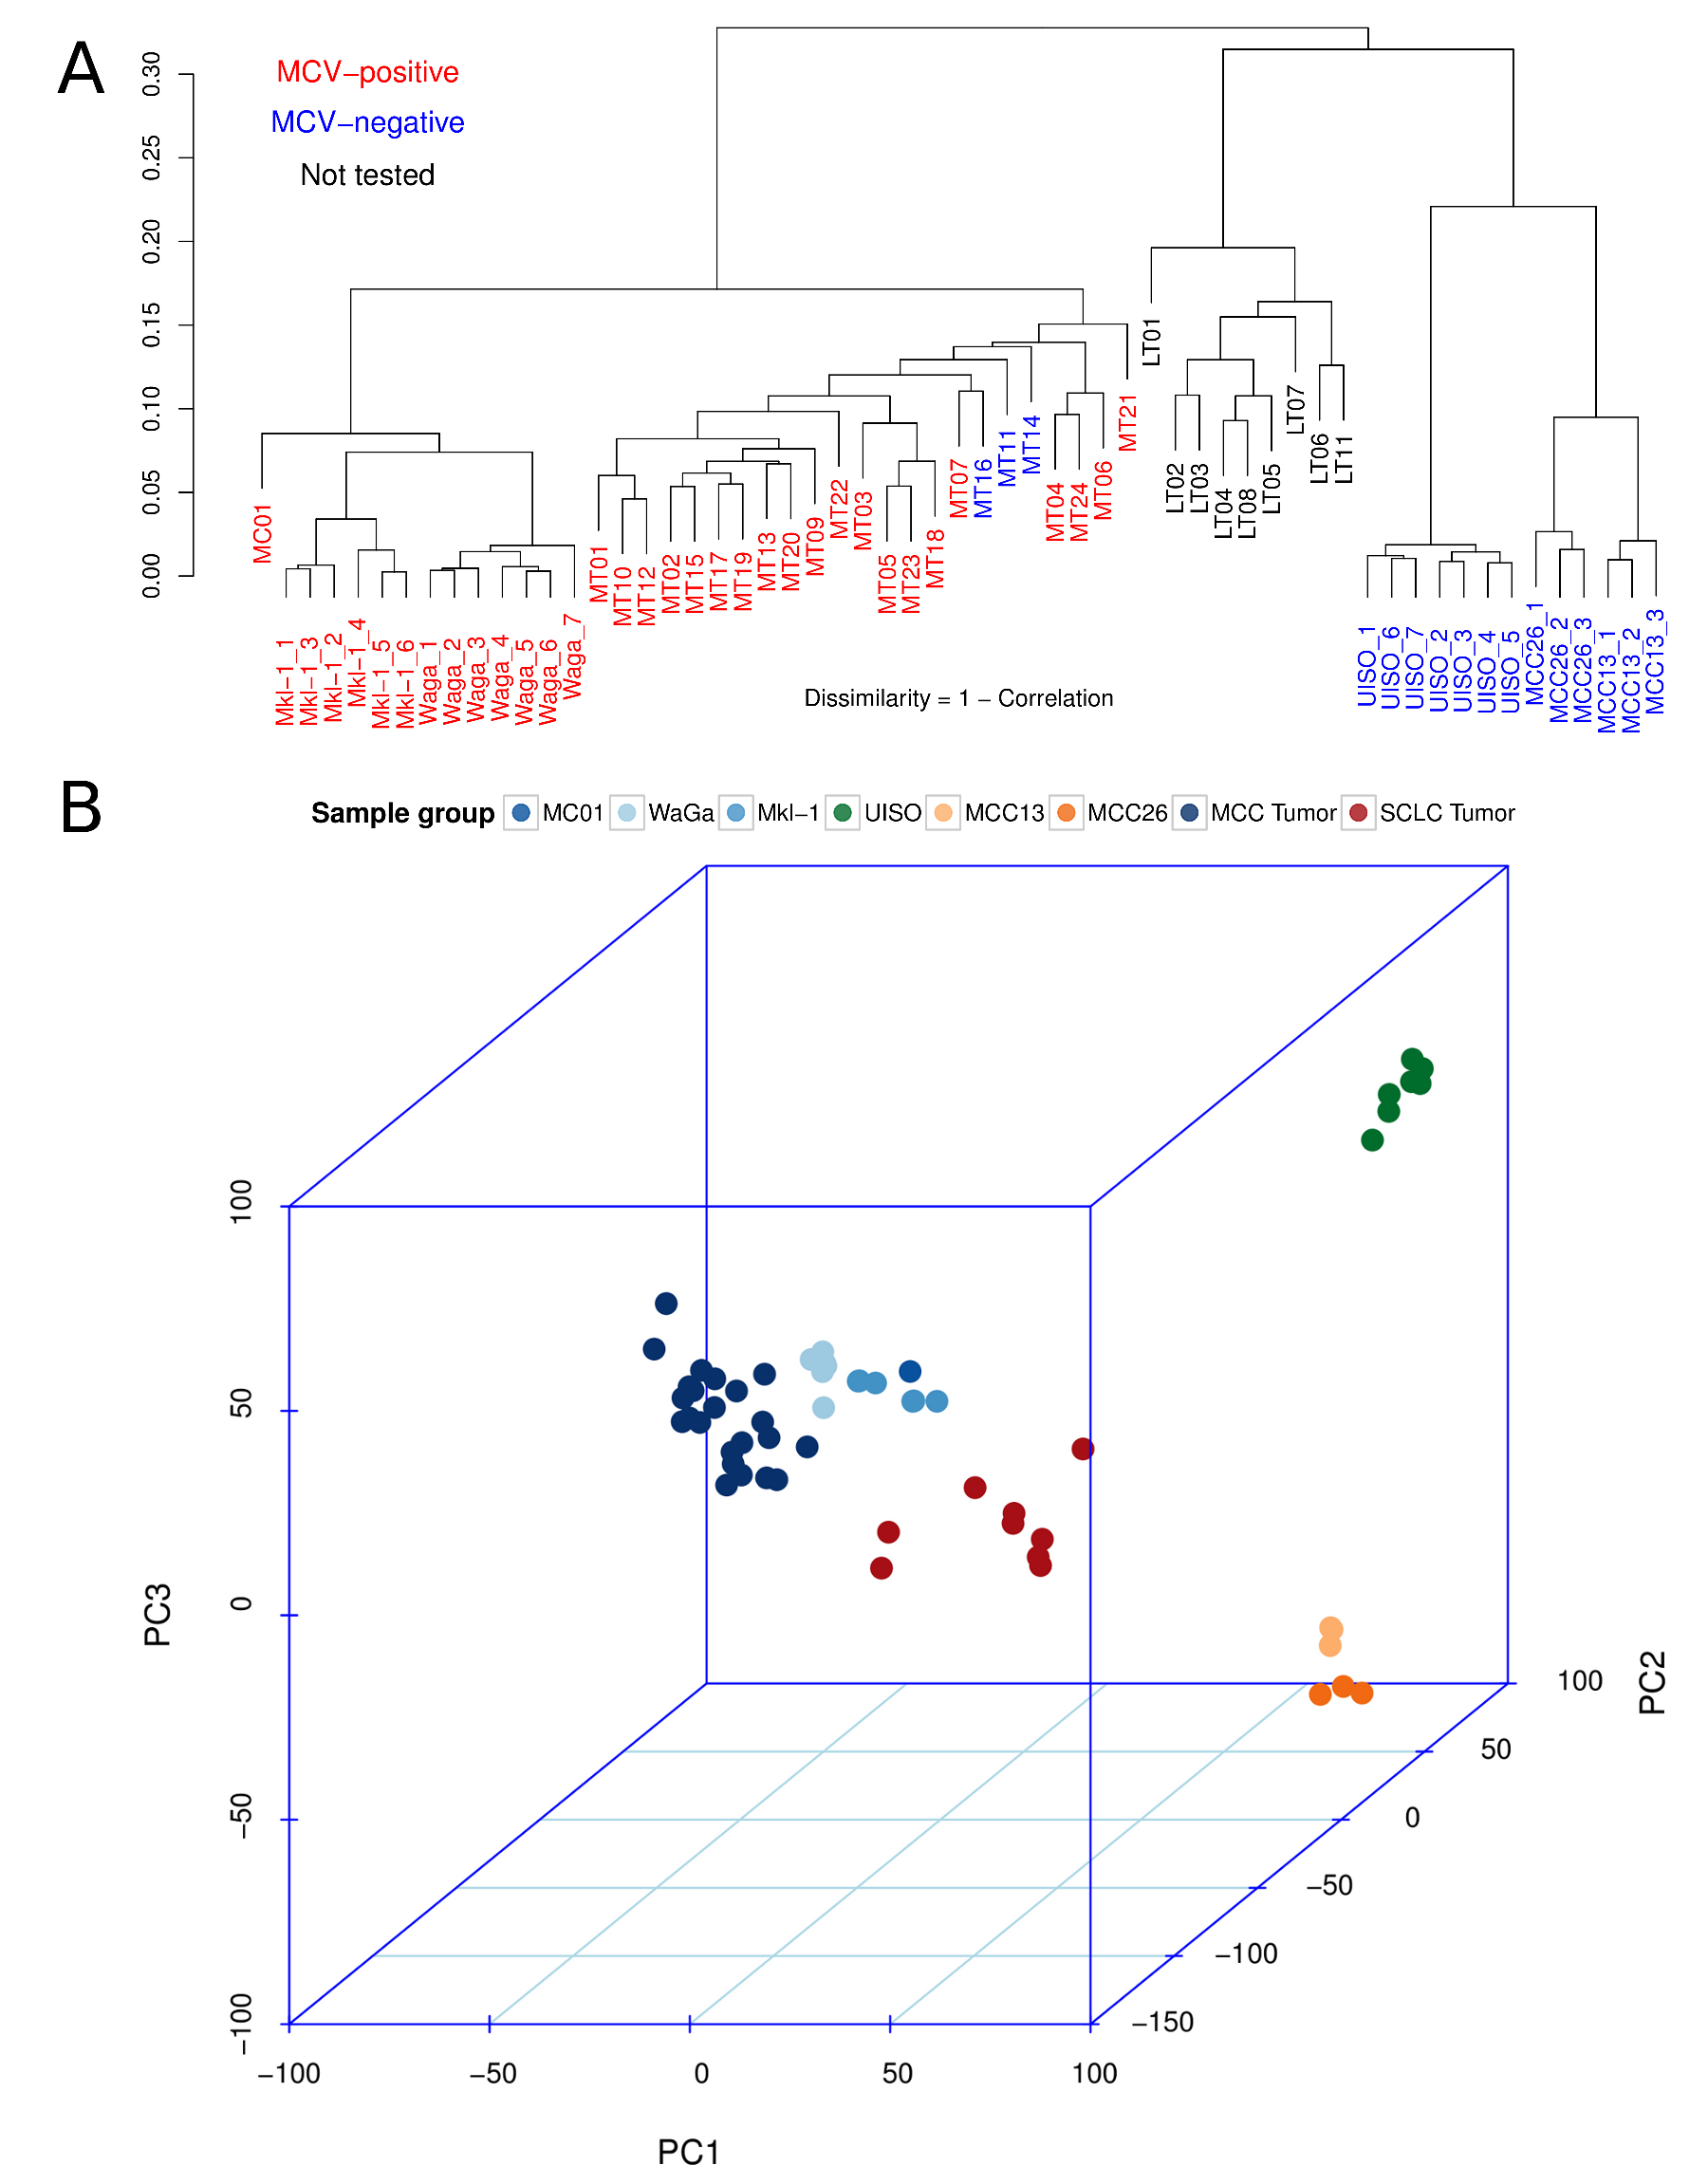
\includegraphics[width=\figwidthoneandhalfcol]{images/fig1}
  \end{center}
  
  \caption{
    {\bf \uline{Variant cell lines} cluster separately from MCC tumors and classic MCC cell lines.}
    A. Hierarchical clustering of microarray expression data from MCC cell lines and MCC and SCLC frozen tumor samples.
    Average linkage was applied for merging clusters to the variance-filtered probe set expression values.
    One minus the Spearman correlation was used as a dissimilarity metric.
    Legend: MCV positive, red; MCV negative, blue; not tested, black.
    B. Principal components analysis of microarray expression data from MCC cell lines and MCC and SCLC tumor samples was performed with variance-filtered probe set expression values for each sample.
    The variance in the expression data accounted for \uline{by the first three principal components are 26\%, 22\%, and 7\%)}.}
  
  \label{fig:clustering}

\end{figure}

\begin{figure}[!ht]

  \begin{center}
    %% 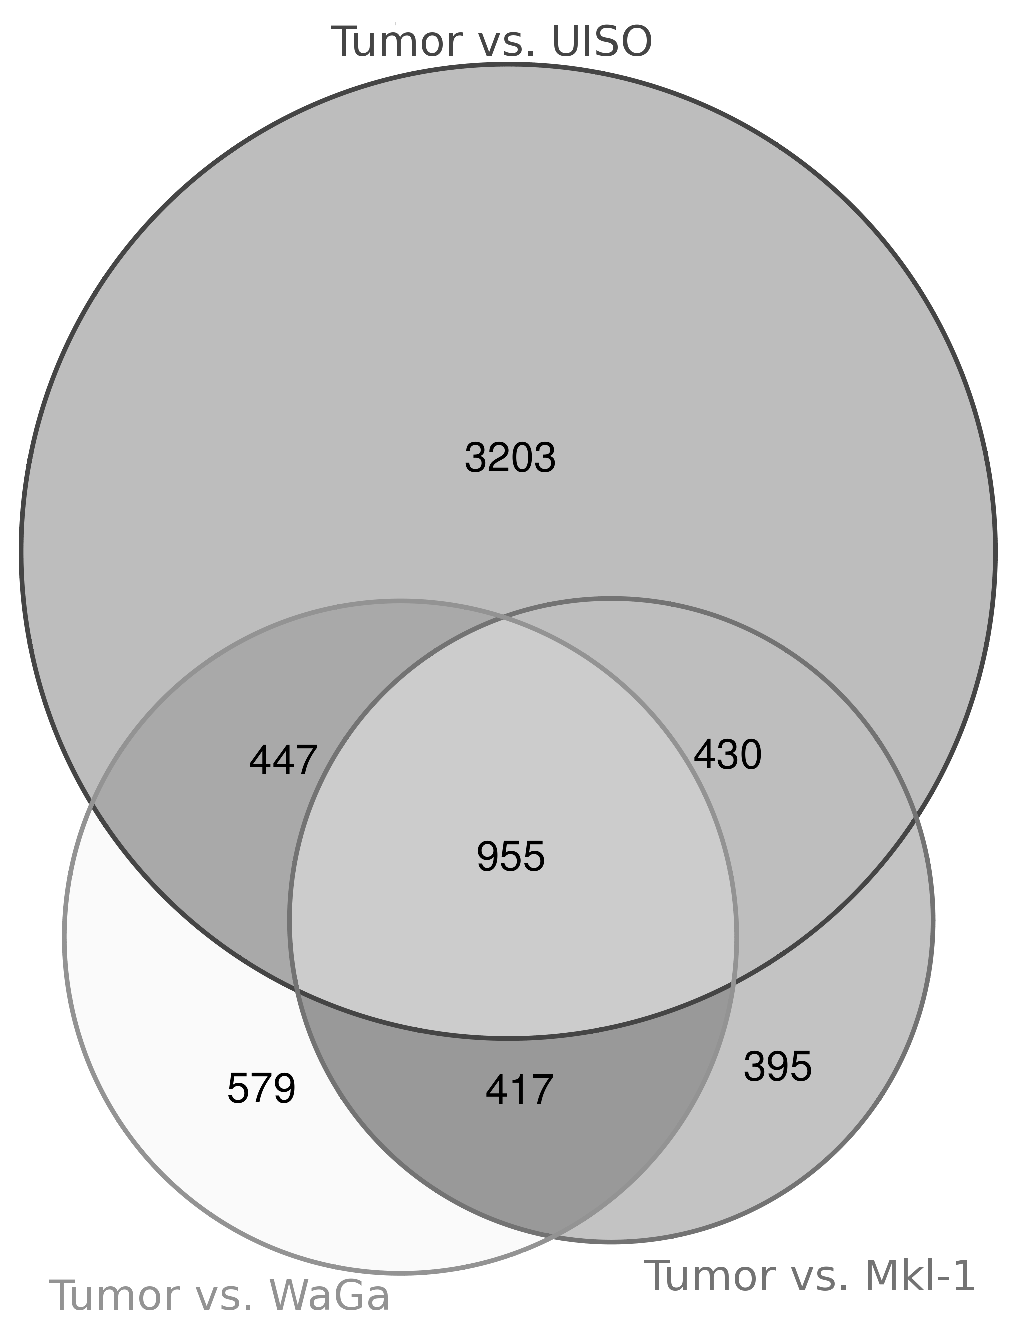
\includegraphics[width=\figwidthonecol]{images/fig2}
  \end{center}

  \caption{
    {\bf Compared to MCC tumors, \uline{variant MCC cell lines} have more differentially expressed genes than classic MCC cell lines.}
    A Venn diagram showing the number of probe sets commonly differentially expressed when comparing the MCC tumor samples to UISO, other \uline{variant (MCC13 and MCC26), and classic (WaGa and Mkl-1) cell lines.}
    Only probe sets with an absolute fold change greater than 2 and a $q$-value less than 0.05 are counted (total: 13,329 probe sets).}

  \label{fig:venn}
\end{figure}


\begin{figure}[!ht]
  \begin{center}
    %% 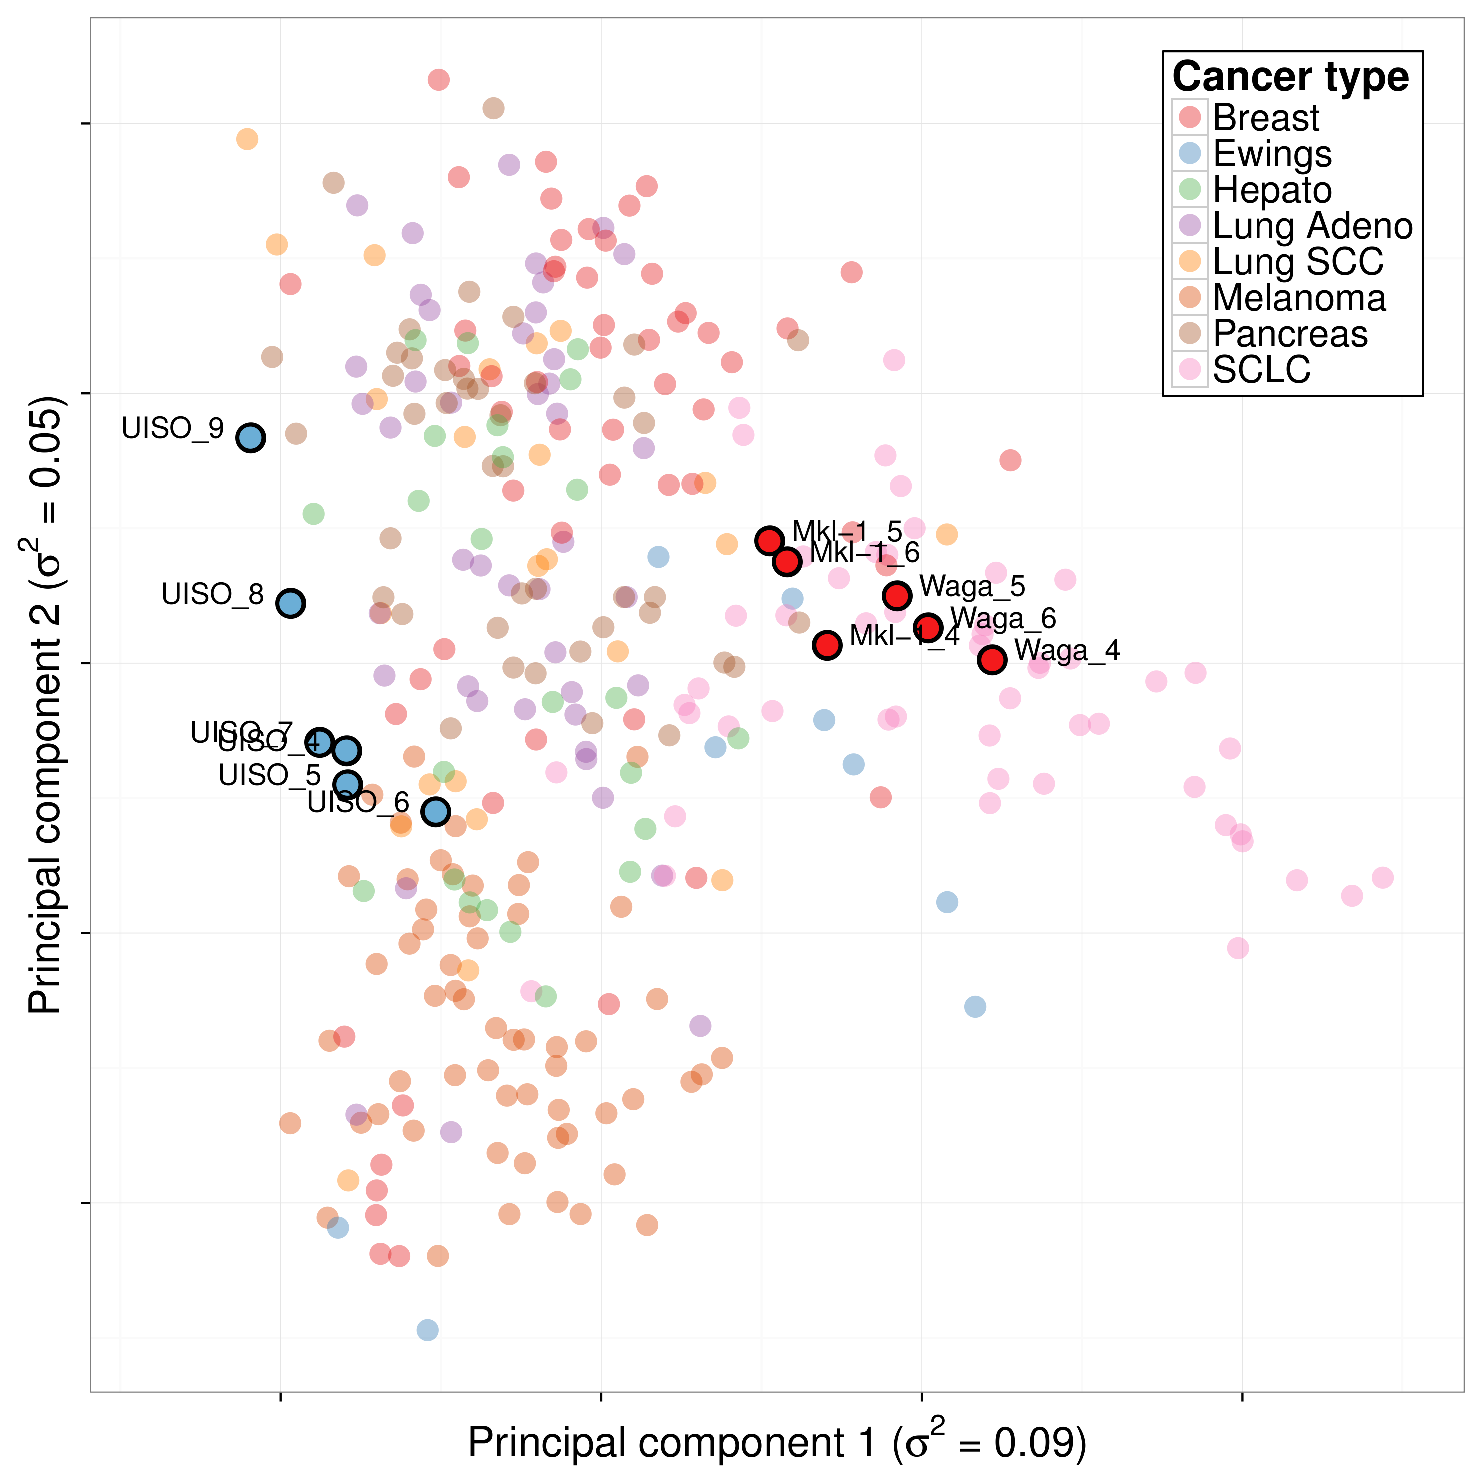
\includegraphics[width=\figwidthonecol]{images/fig3}
  \end{center}

  \caption{
    {\bf Among multiple cancer cell lines, variant cell lines are distinct from classic MCC cell lines} as well as other neuroendocrine lines.
    Principal components analysis of microarray expression data from MCC cell lines and cell lines from the Cancer Cell Line Encyclopedia was computed from variance-filtered probe set expression values for each sample.
    The variance in the expression data accounted for by components one and two are 8\% and 5\%, respectively.}

  \label{fig:pcaccle}
\end{figure}

\begin{figure}[!ht]
  \begin{center}
    %% 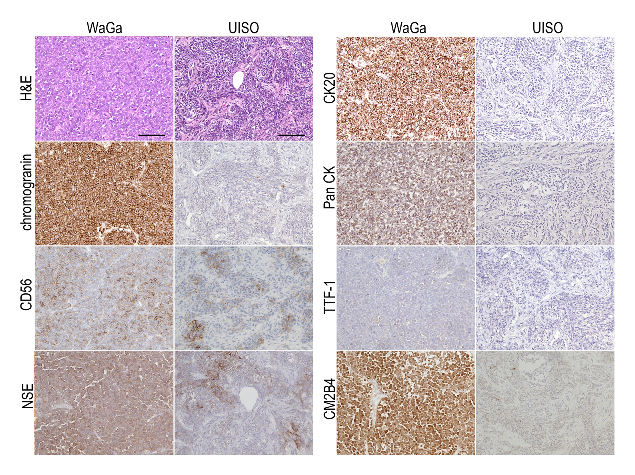
\includegraphics[width=\figwidthoneandhalfcol]{images/fig4}
  \end{center}

  \caption{
    {\bf UISO xenograft tumors are histologically atypical for MCC.}
    Representative images of hematoxylin and eosin staining (H\&E) and immunohistochemical staining of WaGa and UISO xenograft tumors in NOD/Scid mice.
    Scale bar $=100\mu\mathrm{m}$.}

  \label{fig:ihc}
\end{figure}


%% \newpage

\begin{figure}[!ht]
  \begin{center}
    %% \includegraphics[width=\figwidthoneandhalfcol]{images/fig5}
  \end{center}
  
  \caption{
    {\bf Spectral karyotyping (SKY) of metaphase chromosomes confirms the identity of the UISO cell line.} 
    A. Chromosomes stained with DAPI and converted into G-banding-like appearance.
    B. Chromosomes in display colors.
    C. Chromosomes in classification colors.
    D. UISO spectral karyotype (with DAPI and classification images of each chromosome side by side).
    This cell has 46 chromosomes and contains previously described rearrangements, including an insertion at 1p36.2, a cryptic insertion or duplication on 6q, a dicentric chromosome 8, and a small heterogeneous ring chromosome.}

  \label{fig:sky}
\end{figure}

\clearpage

%% \section*{Tables}

%% \begin{table}[H]
%%   \begin{center}

%%     \caption{
%%       \bf{Median correlation values of cell line-tumor comparisons between Merkel cell polyomavirus positive and negative tumor samples.}}
    
%%     \begin{tabular}{rcc}
%%       \hline
%%       & Virus negative & Virus positive\tabularnewline
%%       \hline
%%       WaGa vs. tumor & 0.85 & 0.83\tabularnewline
%%       Mkl-1 vs. tumor & 0.85 & 0.83\tabularnewline
%%       UISO vs. tumor  & 0.66 & 0.66\tabularnewline
%%       \hline
%%       \label{tab:mcvcorr}
%%     \end{tabular}
    
%%   \end{center}
  
%% \end{table}

\clearpage

\begin{table}[H]

  \begin{center}
    
    \caption{
      \textbf{Random forest classification of MCC cell lines.}
      A random forest classifier was trained using the microarray probe set expression data for the 23 MCC and 9 SCLC tumor samples.
      The classifier was then applied to the MCC cell lines, and the average class prediction was determined for each of the MCC cell lines (over sample replicates).
      The class assignment (MCC and SCLC) probability is given as the fraction of trees in the random forest voting for each class.
      The values shown are the average of six replicates for Mkl-1 WaGa,  and UISO, \uline{3 replicates for MCC13 and MCC16,} and 1 replicate of MC01.
    }
    
    \begin{tabular}{rcc}
      \hline 
      & MCC  & SCLC \tabularnewline
      \hline 
      WaGa & \textbf{0.89} & 0.11\tabularnewline
      Mkl-1 & \textbf{0.85} & 0.15\tabularnewline
      MC01 & \textbf{0.83} & 0.17\tabularnewline
      MCC13 &0.43 & \textbf{0.57}\tabularnewline
      MCC26 & 0.40 & \textbf{0.60}\tabularnewline
      UISO & 0.43 & \textbf{0.57}\tabularnewline
      \hline 
      \label{tab:classifier}

    \end{tabular}
    
  \end{center}
  
\end{table}


\end{document}



